  Unfortunately, this endogenous gridpoints solution is not very
  well-behaved outside the original range of gridpoints targeted by
  the solution method.  (Though other common solution methods are no
  better outside their own predefined ranges).
  Figure~\ref{fig:ExtrapProblem} demonstrates the point by plotting
  the amount of precautionary saving implied by a linear extrapolation
  of our approximated consumption rule (the consumption of the perfect
  foresight consumer $\cFuncAbove_{T-1}$ minus our approximation to
  optimal consumption under uncertainty, $\Alt{\cFunc}_{T-1}$).
  Although theory proves that precautionary saving is always positive,
  the linearly extrapolated numerical approximation eventually
  predicts negative precautionary saving (at the point in the figure
  where the extrapolated locus crosses the horizontal axis).

  \hypertarget{ExtrapProblemPlot}{}
  \begin{figure}
    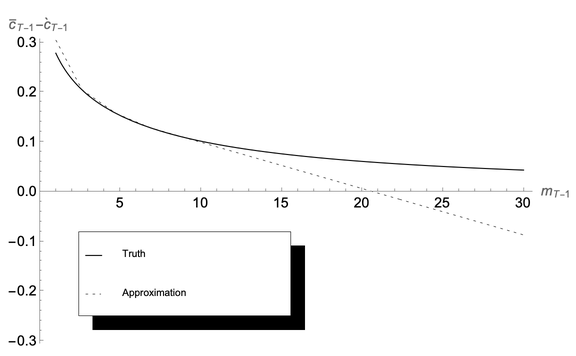
\includegraphics[width=6in]{./Figures/ExtrapProblemPlot}
    \caption{For Large Enough ${m}_{T-1}$, Predicted Precautionary Saving is Negative (Oops!)}
    \label{fig:ExtrapProblem}
  \end{figure}

  This error cannot be fixed by extending the upper gridpoint; in the
  presence of serious uncertainty, the consumption rule will need to be
  evaluated outside of \textit{any} prespecified grid (because starting
  from the top gridpoint, a large enough realization of the uncertain
  variable will push next period's realization of assets above that
  top; a similar argument applies below the bottom gridpoint).  While a judicious extrapolation technique can prevent this
  problem from being fatal (for example by carefully excluding negative
  precautionary saving), the problem is often dealt with using inelegant
  methods whose implications for the accuracy of the solution are
  difficult to gauge.
